% =====================================================================
%  chunks/ch04j.tex —— 原书 p.244–258（PDF 251–265）
%  第 4 章 §5（上）：基本群在拓扑学中的作用；低维流形；纽结；开流形的边界
% =====================================================================
% [原文 p.244]
\begin{corollary*}{}
存在一个 CW 复形 $M$（它同时是一个光滑流形），其上同调群 $H^{3}(M;\Z)$ 中含有 7-挠，并且 $M$ 上存在两个 $\SO$-向量丛 $\eta_{1},\eta_{2}$，使得
\begin{enumerate}[label=(\roman*),leftmargin=2.4em,itemsep=0pt,topsep=2pt]
  \item $p_{2}(\eta_{1})\neq p_{2}(\eta_{2})$；
  \item 向量丛 $\eta_{1},\eta_{2}$ 是 PL 同构的。
\end{enumerate}
\end{corollary*}

这一结果意味着：整 Pontryagin 类的挠部分一般不是 PL 不变的（Milnor--Kervaire，1960 年代初）。

早在 1940 年代就已确立（由 Whitney）：只要 $n\neq 2$，在适当而简单的条件下，浸入 $S^{n}\to M^{2n}$ 可以经正则同伦形变为光滑嵌入。这一结论在例外情形 $n=2$ 下失效；正是这个例外情形，构成了单连通 4 维流形理论最根本的技术困难。从 1950 年代末到整个 1960 年代，多位拓扑学家（Haefliger、Stallings、Levine 等）建立了单连通流形（从同伦球面入手）映入欧氏空间的嵌入理论，所用工具之一就是上面描述的整套流形分类装置。不过我们不在这里阐述这一理论的结果；本丛书将另有一篇专文讨论这一主题，以及 3 维流形与 $\R^{3}$ 中纽结的深刻理论。

\section[基本群的作用。 低维流形。 高维分类理论。 高阶符号差]{基本群在拓扑学中的作用。低维流形（$n=2,3$）。纽结。开流形的边界。有理 Pontryagin 类的拓扑不变性。维数 $\ge 5$ 的非单连通流形的分类理论。高阶符号差。Hermitian $K$ 理论。几何拓扑：非光滑同胚的构造。Milnor 的例子。环带猜想。拓扑结构与 PL 结构}

\takeaway{本节以基本群为线索：先处理 2、3 维流形与纽结的分类（Dehn 扭转、纽结群），再转向高维流形。核心结论是 Novikov 定理（1966）：有理 Pontryagin 类是拓扑不变量，其证明依赖非单连通流形与环状区域上的手术技巧。}

基本群在拓扑学中起着格外重要的作用：它出现在本学科的一切技术装置之中，也同样出现在拓扑方法的一切应用之中。事实上，对低维流形（即维数为 2 或 3 的流形）而言，基本群实质上承载了全部非平凡的拓扑事实。例如读者将会记得，闭曲面 $M^{2}$ 的自同胚的分类——它的同伦类与同痕类（即同伦同胚的类）——按照 Nielsen 的工作，全都归结为考虑 $\pi_{1}(M^{2})$ 的自同构群模去内自同构子群，从而最终归结为「初等」自同构的复合。对亏格为 $g$ 的可定向曲面 $M_{g}^{2}$，$\pi_{1}(M_{g}^{2})$ 的自同构群按通常方式用 $2g$ 个生成元与单个关系
\[
a_{1},b_{1},\dots,a_{g},b_{g};\qquad \prod_{i=1}^{g}a_{i}b_{i}a_{i}^{-1}b_{i}^{-1}=1
\]
给出，它由下列初等自同构生成（Dehn，1920 年代）：

% [原文 p.245]
\begin{align}
\alpha_{i}:&\quad b_{i}\mapsto b_{i}a_{i};\quad b_{k}\mapsto b_{k},\ k\neq i,\quad a_{q}\mapsto a_{q};\quad 1\le i\le g;\notag\\
\beta_{i}:&\quad a_{i}\mapsto a_{i}b_{i};\quad a_{k}\mapsto a_{k},\ k\neq i,\quad b_{q}\mapsto b_{q};\quad 1\le i\le g;\notag\\
\gamma_{i}:&\quad b_{i}\mapsto a_{i+1}^{-1}b_{i}a_{i};\notag\\
&\quad b_{i+1}\mapsto b_{i+1}b_{i}a_{i}^{-1}b_{i}^{-1}a_{i+1};\quad b_{q}\mapsto b_{q},\ q\neq i,i+1; \tag{5.1}\\
&\quad a_{i+1}\mapsto a_{i+1}^{-1}b_{i}a_{i}b_{i}^{-1}a_{i+1}b_{i}a_{i}^{-1}b_{i}^{-1}a_{i+1};\notag\\
&\quad a_{k}\mapsto a_{k},\ k\neq i+1,\quad 1\le i\le g-1;\notag\\
\delta:&\quad a_{j}\mapsto b_{g+1-j};\quad b_{j}\mapsto a_{g+1-j}.\notag
\end{align}

% [Tutor Note: (5.1) 中的 $\alpha_{i},\beta_{i}$ 是沿 $a_{i}$ 或 $b_{i}$ 的换位子型扭转，$\gamma_{i}$ 是 Dehn 扭转；$\delta$ 是互换两组生成元并把下标倒序，它反转曲面的定向，因此 Nielsen 分类必须把自同构群模去内自同构，否则会把定向反转的类混进来。]

注意 $\alpha_{i},\beta_{i},\gamma_{i}$ 保持定向，而 $\delta$ 反转定向。

基本群也决定了纽结理论，即嵌入 $S^{1}\hookrightarrow S^{3}$ 的理论；由这样的嵌入决定的\emph{纽结群}定义为 $\pi_{1}(S^{3}\setminus S^{1})$。这个群有一个特殊元素 $a$，即环路 $S_{\varepsilon}^{1}$ 的类：把嵌入的圆周 $S^{1}$ 沿每一点处垂直于 $S^{1}\subset S^{3}$ 的方向移动一小段距离 $\varepsilon$，使所得的圆周 $S_{\varepsilon}^{1}$ 与原纽结 $S^{1}\subset S^{3}$ 的环绕系数为零。纽结 $S^{1}\subset S^{3}$ 的管状 $\varepsilon$-邻域的边界是一个环面 $T^{2}$，并且可以证明：对非平凡纽结，包含映射
\[
T^{2}\hookrightarrow(S^{3}\setminus S^{1})
\]
以典范的方式决定一个同构于 $\Z\oplus\Z$ 的子群，其生成元也是典范定义的（其中之一正是上面定义的元素 $a$）。

很可能纽结群连同这个典范定义的子群（$\cong\Z\oplus\Z$，带有特异基）构成纽结的完全不变量。特别地，纽结的群同构于 $\Z$ 当且仅当该纽结是平凡的，即嵌入 $S^{1}\hookrightarrow S^{3}$ 同痕于（即可借助 $S^{3}$ 的自微分同胚形变到）平凡嵌入（Papakyriakopoulos 定理，1950 年代末证明）。

然而，群论性质的困难使人无法用这些手段得到判定任一给定纽结是否平凡的算法。Haken 在 1960 年代初用不同的想法构造了这样的算法，但其缺点是它只是「原则上」的算法：算法所需步骤数量极其庞大，使其无法用于实际目的。

% [原文 p.246]
此外还使用着各种别的纽结不变量（其中实际最有用的一个是「Alexander 多项式」），它们最终都由纽结的群决定。对某些目的而言，方便的做法是考虑出现在纽结补集 $S^{3}\setminus S^{1}=U$ 的典范 $\Z$-覆叠 $\tilde U\to U$ 的 $\Z[\Z]$-模同调（见第 3 章 §5）中的不变量。

% [Tutor Note: 这里的 $\Z[\Z]$-模同调是纽结补集无穷循环覆叠上的同调；Alexander 多项式正是该模的挠不变量，所以它「最终由纽结群决定」，但群本身并不等于这些同调数据。]

有一类相对简单的纽结，其纽结补集 $U$ 是底为 $S^{1}$ 的纤维丛，纤维为亏格 $g$ 的带一个穿孔的曲面（$g$ 称为纽结的亏格）：
\[
U\to S^{1},\qquad F\cong M_{g}^{2}\setminus\{*\}.
\]
（任意纽结的亏格，是 $U$ 中以该纽结为边界的曲面的最小亏格。）可以证明：若纽结的补集 $U$ 是纤维丛（如上），则该纽结由 $\C^{2}\supset S^{3}$ 中的一个代数方程定义：
\[
f(z,w)=0,\qquad |z|^{2}+|w|^{2}=\varepsilon>0,
\]
其中 $f(z,w)$ 是多项式，且在 $z=w=0$ 处满足 $f_{z}=f_{w}=0$；一般地，这样的方程决定 $S^{3}$ 中的一个链环，由若干嵌入圆周组成，但解集常常连通，从而表示一个纽结 $S^{1}\subset S^{3}$。用 $f$ 来说，纤维丛 $U$ 本质上由
\[
(z,w)\mapsto\arg f=\varphi,\qquad f=\rho e^{\ii\varphi},\qquad \rho^{2}=\varepsilon
\]
给出。

由 Papakyriakopoulos 的一个定理（1950 年代末），若 $M^{3}$ 是任一满足 $\pi_{2}(M^{3})\neq 0$ 的流形，则存在嵌入的 2-球面 $S^{2}\subset M^{3}$，它在 $M^{3}$ 中不同伦于零。由此可知，对纽结的补集 $S^{3}\setminus S^{1}$，有 $\pi_{i}(S^{3}\setminus S^{1})=0$（$i\ge 2$），于是全部同伦不变量原则上都由 $\pi_{1}$ 决定。

每个有限表示群（即能用有限个生成元与关系给出的群）都可用标准构造实现为某个维数 $\le 2$ 的有限 CW 复形 $K$ 的基本群 $\pi_{1}(K)$，或实现为某个维数 $\le 4$ 的流形 $M$ 的基本群 $\pi_{1}(M)$。

根据 P. S. Novikov、Adyan 与 Rabin（1950 年代初期与中期）关于有限表示群理论中若干问题的算法不可判定性的结果（特别是「任一给定表示是否表示平凡群」这一问题），不难推出以下问题也是算法不可判定的：任一给定的维数 $\ge 2$ 的有限 CW 复形是否同伦等价于某个标准的单连通 CW 复形；同样，任一给定的维数 $\ge 4$ 的闭流形是否同伦等价于某个标准的单连通流形。这一观察是 A. A. Markov（1950 年代末）作出的；他还证明了（这一点更难）：对每个维数 $\ge 4$ 的流形，它是否同胚（或 PL 同胚、或微分同胚）于某个标准的单连通流形，也同样是算法不可判定的。CW 复形的可缩性在维数
% [原文 p.247]
$\ge 3$ 时是算法上不可识别的性质；而「维数 $n\ge 5$ 的闭流形是否同胚于 $n$-球面 $S^{n}$」这一问题同样是不可判定的；这些不可判定性结果由 S. P. Novikov 在 1960 年代初用同调代数方法建立；很可能后一问题在 $n=4$ 时也仍不可判定。另一方面请注意：有限 2 维 CW 复形的同胚问题，以及「给定的带边 3 维流形是否同胚于可缩流形」的问题，都极可能是算法可解的。后一问题在算出带边 3 维流形边界的亏格之后，归结为识别 $S^{3}$ 的同伦型。闭 3 维流形与纽结理论中最简单的算法问题看来也是可解的；不过，正如识别平凡纽结的问题（见上文）所表明的，尽管算法存在，问题在实践中仍可能难以处理。至于球面 $S^{3}$ 的识别问题，在亏格 $g=2$ 的 Heegaard 图类中已有算法解决（Birman、Hilden，1960 年代末）。\footnote{在其近作 \emph{The solution to the recognition problem for $S^{3}$}（以色列海法，1992 年 5 月）中，H. Rubinstein 声称构造了识别 3 维球面的算法。本综述的作者不知道该文中的论证是否都经过验证。}

有可能对某些 3 维问题存在高效、足够快的算法，例如识别平凡纽结或球面 $S^{3}$ 的问题；这里的「足够快」是指：这类算法虽不总是严格适用，却「实际上总能」快速解决问题。对实际目的而言，这样的算法比那些永远适用但只「原则上」适用的算法更有用。这方面值得提及一项数值实验（记录在生物物理文献中）：它联系着对某些物质性质的研究，例如具有长的闭合分子（「链环化」的分子）在纽结与链环构形下的性质（Frank--Kamenetskiĭ 等，1970 年代）；类似的结构在物理学的其他领域也遇到过。最后我们指出：在交叉数不太大时，纽结可以通过其 Alexander 多项式被有效且唯一地识别。\footnote{1980 年代末，V. Jones 发现了纽结的若干引人注目的新多项式不变量，使纽结理论中某些经典问题得以解决。其想法来自：把纽结的等价类表示为不同群中的共轭类（这些群经「Markov 移动」彼此等价），以及来自数学物理中 Yang--Baxter 理论的辫群表示；由此得到统计物理与量子物理中某些 2 维模型的精确解。在 Jones 的工作之后，多位拓扑学家、代数学家与数学物理学家进一步发展了这一理论。（例如可参看 Kauffman, Louis H., \emph{Knots and physics}. Singapore: World Scientific, 1994，Series on knots and everything；或 Dror Bar--Natan 的讲义 \emph{Lectures on Vassiliev invariants}。）现在这一理论已在 A. Schwarz 与 Witten 所创的「拓扑量子场论」这一更现代的框架下重新表述。（另见附录。）}

关于 $S^{3}$ 是唯一单连通闭 3 维流形的 Poincaré 猜想，至今仍未获证明。1950 年代末 Milnor 证明：由上述定理（断言在 $\pi_{2}(M^{3})\neq 0$ 的流形 $M^{3}$ 中存在同伦
% [原文 p.248]
非平凡的嵌入 2-球面 $S^{2}\subset M^{3}$），可以推出：闭 3 维流形分解为下列三种初等类型的 3 维流形的连通和（连通和的定义见上文 §4），这一分解在同伦等价意义下是唯一的：

\textbf{类型 I}：$\pi_{1}$ 有限的流形；

\textbf{类型 II}：$\pi_{2}=0$ 的流形；

\textbf{类型 III}：$M^{3}=S^{2}\times S^{1}$。

并且，若 Poincaré 猜想成立，则该分解在拓扑意义下唯一。

类型 I 的流形可通过 $S^{3}$ 上 $SU_{2}$ 或 $SO_{4}$ 的有限子群自由作用（即没有非平凡元素固定任何点）的商来构造。类似地，类型 II 的流形可作为 3 维 Lobachevski 空间 $L^{3}$ 的运动离散群 $G$（$G\subset O_{3,1}$）的自由作用、且基本区域紧致的轨道空间而得到。从 1960 年代中期到 1980 年代初，V. S. Makarov 造出了若干无穷系列的这类流形；不过这些例子尚未被详细研究。\footnote{1980 年代中期，Fomenko 与 Matveev 借助计算机，利用 3 维流形的「复杂度理论」（Matveev）构造了一批漂亮的常（规范化的）负曲率闭 3 维流形。其中一个流形的体积竟然小于 Thurston 猜测为极小的某个 3 维流形。} Thurston 数年前开始的 3 维流形研究的大规模纲领，只在较窄的 Haken 流形类中完成。该纲领导致「几何化猜想」的提出；此猜想若成立，将有以下优美结果作为推论：若闭 3 维流形 $M$ 满足 $\pi_{2}(M)=0$，且 $\pi_{1}(M)$ 没有除 $\Z$ 以外的非平凡阿贝尔子群，则 $M$ 同伦等价于一个常负曲率的紧致 3 维流形，从而其基本群同构于 Lobachevski 3 空间的一个离散等距群，且基本区域紧致。与此纲领相关的是如下猜想：若 $\pi_{1}(M^{3})$ 无限且 $\pi_{2}(M^{3})=0$，则流形 $M^{3}$ 同伦等价于一个常负曲率的 3 维流形，因而可作为 $L^{3}$ 的某个离散运动群的轨道空间得到。

% [Tutor Note: 这里 $L^{3}$ 是双曲 3 空间，$O_{3,1}$ 是它的（Lorentz）等距群；「常负曲率」即双曲结构。注意类型 II 的构造要求群在 $L^{3}$ 上自由作用且基本区域紧致，二者的区别正是 Thurston 几何化纲领里「几何化」与「模型几何」的差别。]

下面转向高维流形（维数 $n\ge 5$）的拓扑问题。考虑 Pontryagin 类的拓扑不变性问题：$p_{k}\in H^{4k}(M^{n};\Q)$ 取有理（或实）上同调，问题在于 $p_{k}$ 沿闭链的积分在同胚下不变（这里把 Pontryagin 类表示为微分形式，或许用相对某个 Riemann 度量的曲率张量来表达）。乍看之下，这个问题与基本群毫无关系；事实上，在解决该问题时可以不失一般性
% [原文 p.249]
地假定流形 $M^{n}$ 单连通。因此，Novikov 在 1960 年代中期给出的（肯定的）解答诉诸非单连通的环状区域以及非单连通流形特有的技巧，初看显得人为。然而迄今没有找到别的证明。此外，引入环状区域、以便把关于同胚的问题归约为关于非单连通流形的光滑或 PL 拓扑的辅助问题，这一手法首先由 Kirby 作了实质性发展，用来证明所谓的「环带猜想」（最终由 Siebenmann、Hsiang、Shaneson、Wall 与 Casson 在 1960 年代末解决）；后来它又被进一步提炼为求解纯粹拓扑流形及其间同胚的拓扑问题的工具（由 Kirby、Siebenmann、Lashof 与 Rothenberg 完成）。

除符号差公式之外，对单连通流形而言，Pontryagin 类与数之间实质上不存在其他同伦不变的关系。（根据 Thom 与 Wu 关于类 $w_{i}$ 与 $p_{k}$ 的定理，可能的同伦不变量只有模 2 的某些示性数（对类 $w_{i}$）与模 12 的某些示性数（对类 $p_{k}$），以及若干其他示性数。有理 Pontryagin 类 $p_{k}$ 一般不是同伦不变量这一事实，是 Serre--Rohlin 定理（关于群 $\pi_{n+3}(S^{n})$ 对 $n\neq 4$ 有限）的一个相对直接的推论（正如 Dold 在 1950 年代中期所观察到的那样）。最简单的例子来自底为 $S^{4}$、纤维为 $S^{2}$ 的一族 $\SO_{3}$-向量丛，每个这样的丛由类 $p_{1}\in H^{4}(S^{4};\Z)$（$\cong\Z$）（或由 $\pi_{3}(\SO_{3})\cong\Z$ 的一个元素）决定。由同态
\[
J\colon\pi_{3}(\SO_{3})\to\pi_{6}(S^{3})\cong\Z_{12}
\]
的像的有限性可以推出：这些向量丛的全空间只落入有限多个同伦型（同伦型的判定达到 Dold 所定义的「纤维同伦等价」意义下的丛类）。事实上这样的丛有无穷多个，且其 Pontryagin 类 $p_{1}$ 各不相同，因此至多只有 $p_{1}\pmod{48}$ 可能在「这些丛的全空间」这一类流形中是同伦不变量。Browder 与 Novikov 的定理（见上文 §4）表明：即使对一个具体的单连通流形，除符号差的 Hirzebruch--Thom--Rohlin 公式之外，Pontryagin 类之间也不存在同伦不变的关系。

% [Tutor Note: 注意 $J$ 同态的定义域是 $\pi_{3}(\SO_{3})\cong\Z$，像落在有限群 $\pi_{6}(S^{3})\cong\Z_{12}$；正因像有限，无穷多个 $p_{1}$ 不同的丛全空间只有有限多个同伦型，所以 $p_{1}$ 不能是同伦不变量，只剩下模 48 的候选。]

Thom、Rohlin 与 Schwarz 在 1950 年代末证明：有理 Pontryagin 类 $p_{k}$ 在 PL 同胚下不变；他们据此提出了这些类的如下组合定义。对每个闭链 $z\in H_{4k}(M^{n};\Q)$，若它能实现为具有平凡法丛的子流形 $M^{4k}\subset M^{n}$，即
% [原文 p.250]
\begin{align}
M^{4k}\times\R^{n-4k}&\hookrightarrow M^{n},\notag\\
i_{*}([M^{4k}])&=z, \tag{5.2}
\end{align}
则令（参看 Hirzebruch 公式 (3.19)）
\begin{equation}
\langle L_{k}(p_{1},\dots,p_{k}),z\rangle=\tau(M^{4k}). \tag{5.3}
\end{equation}
现在可以援引一般的范畴性质来证明：$L_{k}(p_{1},\dots,p_{k})$ 在这些闭链 $z$ 上的值决定了它在整个 $H_{4k}(M^{n};\Q)$ 上的值。由 Hirzebruch 多项式的形状，有
\begin{equation}
L_{k}=\frac{2^{2k}(2^{2k-1}-1)B_{k}}{(2k)!}\,p_{k}+\tilde L_{k}(p_{1},\dots,p_{k-1}), \tag{5.4}
\end{equation}
其中 $B_{k}$ 是第 $k$ 个 Bernoulli 数；由此可知类 $p_{k}$ 可用 $L_{1},\dots,L_{k}$ 表达：
\begin{equation}
p_{k}=p_{k}(L_{1},\dots,L_{k}). \tag{5.5}
\end{equation}

% [Tutor Note: (5.4) 中 $B_{k}$ 取 $B_{1}=\frac{1}{6}$ 的约定，于是 $k=1$ 时 $L_{1}=\frac{1}{3}p_{1}$，符号差定理即 $\tau(M^{4})=\frac{1}{3}p_{1}$；若误用 $B_{1}=-\frac{1}{2}$ 的另一约定，符号差公式会差一个符号。]

基于类 $p_{k}$ 的这一「符号差」定义，可以对其性质作组合处理。若 $M^{n}$ 是 PL 流形，而 $f\colon M^{n}\to S^{n-4k}$ 是充分细的三角剖分下的单纯映射，则对 $S^{n-4k}$ 的任意最高维单形 $\sigma^{n-4k}$ 的任一内点 $x$，其完全原像具有形式
\[
f^{-1}(x)=M^{4k},\qquad f^{-1}(\operatorname{Int}\sigma^{n-4k})=\operatorname{Int}\sigma^{n-4k}\times M^{4k},
\]
其中 $M^{4k}$ 是 $M^{n}$ 的 PL 子流形。现在我们定义
\[
\langle L_{k}(p_{1},\dots,p_{k}),z\rangle=\tau(M^{4k}),
\]
其中 $z$ 是由 PL 子流形 $M^{4k}\subset M^{n}$ 表示的 $H_{4k}(M^{n};\Q)$ 的元素；然后如前用公式
\[
p_{k}=p_{k}(L_{1},\dots,L_{k})
\]
定义 Pontryagin 类 $p_{k}$。如前面一样，可以证明这确定了 $p_{k}$ 在 $H_{4k}(M^{n};\Q)$ 上的值，从而给出有理 Pontryagin 类 $p_{k}$ 的一个 PL 不变的定义。我们看到，这一提法的背后是光滑映射的横截正则性在 PL 映射情形下的自然而简单的类比。

注意这个定义是非局部的，这与光滑情形相反：在光滑情形，类 $p_{k}$ 用曲率张量表达。类 $p_{k}$ 的局部 PL 表示的存在性已被证明（由 I. M. Gel'fand、Losik 与 Gabrielov 在 1970 年代中期），但迄今还没有有效的（即构造性的）局部定义。

下面我们略述流形 $M^{n}$ 的有理 Pontryagin 类的拓扑不变性的证明。首先注意，不同的光滑
% [原文 p.251]
（或 PL）结构，按同胚的定义，必定具有 $M^{n}$ 的相同的基本开集族（其中每个开集相对于叠置在 $M^{n}$ 上的各种光滑或 PL 结构都是光滑（或 PL）流形）。流形 $M^{n}$ 的有理 Pontryagin 类 $p_{k}$，更确切地说，它们沿 $M^{n}$ 的各个闭链的积分，可以表示为 $M^{n}$ 的某些开的「环状」区域及其覆叠空间的同伦不变量；由此即可推出它们对整个流形 $M^{n}$ 的拓扑不变性。（这里用的是上面通过符号差给出的 $p_{k}$ 的定义。）

于是，首先考虑环面邻域的一个固定嵌入
\[
\R\times T^{n-4k-1}\hookrightarrow\R^{n-4k},
\]
以及 $M^{n}$ 中相应的「环状」区域
\begin{equation}
U^{n}=M^{4k}\times T^{n-4k-1}\times\R\hookrightarrow M^{n}. \tag{5.6}
\end{equation}

相对于 $M^{n}$ 上的光滑（或 PL）结构，这个区域未必是光滑直积；这里重要的是：该区域同伦等价于流形 $M^{4k}\times T^{n-4k-1}$，并且符号差 $\tau(M^{4k})$ 可以表示为这个区域或其覆叠空间的一个同伦不变量，用其上同调环来表达。可以不失一般性地假定流形 $M^{n}$、$M^{4k}$ 单连通，且 $k>1$，$n<8k$。用微分拓扑的方法可以证明：对基本群是自由阿贝尔群的流形，下述断言成立：若 $W^{m}$（$m\ge 6$）是这样的流形（即 $\pi_{1}(W^{m})$ 是自由阿贝尔群），其上定义了群 $\Z$ 的自由连续或光滑作用，使得轨道空间 $W^{m}/\Z$ 是闭流形，且具有底为 $S^{1}$ 的纤维丛 $V^{m}\to S^{1}$ 的同伦型，则流形 $W^{m}$ 微分同胚于一个闭流形与实直线的直积：
\[
W^{m}=N^{m-1}\times\R.
\]
（事实上，要得到这一结论，只需带自由 $\Z$-作用的流形 $W^{m}$ 同伦等价于有限 CW 复形，且轨道空间 $W^{m}/\Z$ 紧致；此外，关于 $\pi_{1}(W^{m})$ 的条件还可以减弱为要求 Grothendieck 群 $K_{0}(\pi_{1})$（见下文）平凡：$K_{0}(\pi_{1})=0$。）

由这个引理，有理 Pontryagin 类的拓扑不变性可如下推出：先把引理用于区域 $U^{n}$（即取 $W^{m}=U^{n}$，$m=n$），赋予其任一光滑结构，并令 $\Z$ 按自然方式作用：
\[
T\colon(x,t)\mapsto(x,t+1),
\]
其中 $x\in M^{4k}\times T^{n-4k-1}$，$t\in\R$。由于 $\pi_{1}(M^{4k})=0$，可知 $\pi_{1}(U^{n})$ 是自由阿贝尔群，于是由上述引理存在微分同胚
% [原文 p.252]
\begin{equation}
U^{n}\cong V^{n-1}\times\R, \tag{5.7}
\end{equation}
其中 $V^{n-1}$ 同伦等价于 $M^{4k}\times T^{n-4k-1}$。由于直积分解 (5.7) 是光滑的，对 Pontryagin 类有
\[
p_{j}(U^{n})=p_{j}(V^{n-1}),\qquad j=1,2,\dots
\]
考虑由环面的 $\Z$-覆叠所决定的 $V^{n-1}$ 的 $\Z$-覆叠空间：
\[
T^{n-4k-2}\times\R\xrightarrow{\ \Z\ }T^{n-4k-1},\qquad
\check V^{n-1}\xrightarrow{\ \Z\ }V^{n-1};
\]
这里 $\check V^{n-1}$ 具有 $M^{4k}\times T^{n-4k-2}$ 的同伦型。再把上述程序用一次，这次让 $\check V^{n-1}$ 扮演 $W^{m}$ 的角色，便得到
\begin{equation}
\check V^{n-1}\cong V^{n-2}\times\R,\qquad V^{n-2}\sim M^{4k}\times T^{n-4k-2}, \tag{5.8}
\end{equation}
\[
p_{j}(V^{n-2})=p_{j}(V^{n-1})=p_{j}(U^{n}),\qquad j\ge 1.
\]
迭代这一论证，最终得到
\begin{equation}
\check V^{4k+1}\cong V^{4k}\times\R, \tag{5.9}
\end{equation}
\[
p_{j}(V^{4k})=p_{j}(V^{4k+1})=\dots=p_{j}(U^{n}),\qquad j\ge 1,
\]
其中 $V^{4k}$ 是光滑闭流形，同伦等价于 $M^{4k}$。符号差公式给出
\[
\tau(M^{4k})=L_{k}(M^{4k})=L_{k}(V^{4k})=\langle L_{k}(p_{1},\dots,p_{k}),[M^{4k}]\rangle,
\]
其中 Pontryagin 类用流形 $U^{n}$ 上任一光滑结构来定义。由此立即推出有理 Pontryagin 类的拓扑不变性。

当 $n\ge 8k$ 时，上述论证给出一个光滑嵌入 $V^{4k}\times\R^{n-4k}\hookrightarrow U^{n}$，不过 $U^{n}$ 带有的光滑结构可能不同；由此得到微分同胚
\[
V^{4k}\times\R^{n-4k}\to M^{4k}\times\R^{n-4k},
\]
其中后一个流形带有任一光滑结构。在上述证明发表后不久，Siebenmann 通过对论证作更细致的分析，证明了即使在不稳定维数 $n<8k$ 的情形这一结论也成立。

对非单连通的闭流形，有理 Pontryagin 类沿某些闭链的积分之间存在非平凡的同伦不变关系；这类关系最简单的例子如下：

% [原文 p.253]
\begin{example*}{1}
设 $n=4k+1$，$z\in H_{4k}(M^{n})$。考虑 $\Z$-覆叠投影 $p\colon\hat M^{n}\to M^{n}$，使得 $p_{*}\pi_{1}(\hat M^{n})$ 恰好由那些与闭链 $z$ 的相交指数为零的闭链 $\gamma$ 组成：
\[
p_{*}\pi_{1}(\hat M^{n})\circ z=0.
\]
存在一个可用同伦不变方式定义的闭链 $\hat z\in H_{4k}(\hat M^{n})$，
使得 $p_{*}\hat z=z$。
\begin{center}
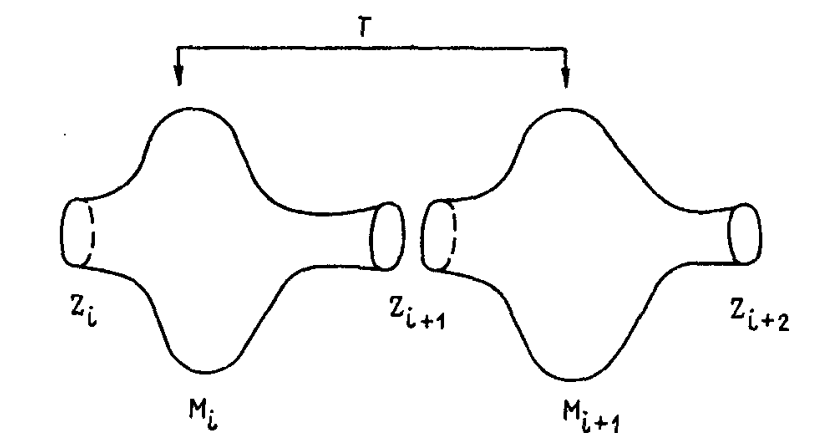
\includegraphics[width=0.7\textwidth]{figures/fig4_28.png}
\end{center}
\figtitle{4.28}{}
在上同调环 $H^{*}(\hat M^{n};\Q)$ 中，我们有一个由
\begin{equation}
\langle x,y\rangle=\langle xy,\hat z\rangle=\langle y,x\rangle, \tag{5.10}
\end{equation}
定义在 $H^{2k}(\hat M^{n};\Q)$ 上的双线性形式，它具有有限维承载子（即使每个元素都零化它的子空间具有有限余维）。把这一双线性形式的符号差记作 $\tau(\hat z)$，则有如下公式：
\begin{equation}
\langle L_{k}(p_{1},\dots,p_{k}),z\rangle=\tau(\hat z). \tag{5.11}
\end{equation}
\end{example*}

\begin{example}{2}
若光滑流形 $V^{4k+q}$ 具有形如 $M^{4k}\times T^{q}$ 的直积的同伦型：
\[
V^{4k+q}\sim M^{4k}\times T^{q},
\]
则可用证明类 $L_{k}(p_{1},\dots,p_{k})$ 的拓扑不变性时所用的技巧，建立如下公式（属 Novikov，1960 年代中期）：
\[
L_{k}(V^{4k+q})=\tau(M^{4k}).
\]
\end{example}

关于「高阶符号差」（higher signature）的一般猜想如下：正如 Hopf（1940 年代初）已经表明的，每个 CW 复形 $K$ 都有一组由 $\pi_{1}(K)$ 完全决定的特殊上同调类，即典范映射 $f\colon K\to K(\pi,1)$ 的诱导同态
% [原文 p.254]
\[
f^{*}\colon H^{*}(K(\pi,1))\to H^{*}(K)
\]
（系数任意）的像。（Hopf 在 2 维情形描述了这些类。）空间 $K(\pi,1)$ 的同伦型及其上同调 $H^{*}(K(\pi,1))$（系数任意，包括 $\Z[\pi]$-模）的代数刻画，由 Eilenberg 与 MacLane 在 1940 年代中期给出；他们随后把群 $\pi$ 的上同调 $H^{*}(\pi)$ 定义为 $H^{*}(K(\pi,1))$。（稍后，D. K. Faddeev 独立地也给出了这些代数对象的定义，其动机来自代数数论。）事实上，这一概念构成了同调代数的基础；同调代数后来由 Cartan、Eilenberg、Serre、Grothendieck 等人推广到模与更一般的阿贝尔范畴的框架中。（这样一种推广——推广到 $A$-模范畴——曾用于上文第 3 章 §6、§7、§9，作为稳定同伦论的代数装置的一部分。）% [Tutor Note: 原书这里的 $K(\pi,1)$ 就是 Eilenberg--MacLane 空间，$H^{*}(\pi)$ 是群上同调；注意上标星号表示上同调，而下一句的 $Df^{*}H^{*}$ 用的是 Poincaré 对偶 $D$ 把它送进同调，次数会变：$H^{j}(\pi;\Q)\to H_{n-j}(M^{n};\Q)$。]

当然，相应地有（闭流形 $M^{n}$ 的）闭链类
\[
Df^{*}H^{*}(\pi;\Q)\subset H_{*}(M^{n};\Q).
\]
于是，「关于高阶符号差的猜想」是：对 $Df^{*}H^{*}(\pi;\Q)$ 中每个维数为 $4k$ 的闭链 $z$，Pontryagin--Hirzebruch 类沿该闭链的积分
\[
\langle L_{k}(p_{1},\dots,p_{k}),z\rangle
\]
应当是同伦不变的。对 $n=4k+1$ 与任意的 $\pi=\pi_{1}(M^{4k+1})$，余维数为 1 的特殊闭链 $z\in H_{4k}(M^{4k+1};\Q)$ 恰好就是那些使公式 (5.11) 关于由 (5.10) 定义的双线性形式成立者，而且这类闭链的相交也具有这一性质。（在 $\pi$ 是自由阿贝尔群的情形，所有闭链都是这种形式。）关于这种余维数 1 的闭链相交的高阶符号差猜想，在两个闭链相交的情形由 Rohlin 解决（1960 年代后半期），随后（1960 年代末）由 Kasparov、Hsiang 与 Farrell 对任意多个闭链的相交解决：
\[
z=D(y_{1}\wedge\dots\wedge y_{k}),\qquad y_{j}\in H^{1}(M^{n};\Q).
\]

这一命题的一个解析证明（用椭圆算子理论）由 Lusztig 在 1970 年代初得到；他还对 $\pi$ 是常负曲率对称空间的运动群的离散子群的情形，对某些闭链建立了该猜想。对阿贝尔的 $\pi$，他首次使用了与该群的有限维表示（及其特征）相联系的一族椭圆复形；对非阿贝尔的 $\pi$，他得以利用 $\pi$ 在 Hilbert 空间 $H_{i}$ 上的酉算子环中的无穷维「Fredholm」表示 $\rho_{i}\colon\pi\to\Aut H_{i}$。（一对酉表示 $\rho_{1},\rho_{2}$ 连同 Noether 算子 $F\colon H_{1}\to H_{2}$，若 $F\rho_{1}-\rho_{2}F$ 是紧算子，则称为\emph{Fredholm 表示}；参看第 1 章末尾。）结果表明，借助带 Fredholm 表示的椭圆算子的指标所满足的 Atiyah--Hirzebruch--Singer 型公式的类比（这类表示用正曲率紧流形的几何来构造，以便定义诸如「带表示的系数的符号差」这样的量），
% [原文 p.255]
高阶符号差猜想可以对一切能实现为对称空间的、基本区域紧致的运动离散群的群 $\pi$ 完全建立（Mishchenko，1970 年代初）。这一结果在 1970 年代由 Solov'ev 等人推广；现在看来，这些方法已经发展到足以证明该猜想对李群的一切离散子群成立的程度（Kasparov，1980 年代初）。\footnote{在这方面，过去十年间用拓扑方法与解析方法得到了许多深刻的结果。特别地，Novikov 的猜想已对 Gromov 引入的「双曲群」以及某些其他群类得到验证，完成者包括 Cohn、Pedersen、Gromov、Rosenberg 等多人。配边论对正标量曲率流形理论的一些漂亮应用，由 Gromov、Lawson、Kreck 与 Stolz 发现并发展。这里，在非单连通情形，类似于高阶符号差、但把 $L$-亏格换成 $A$-亏格的示性数起重要作用。}

在这方面值得注意的是：上述「Fredholm 表示」最初由 Atiyah 在 1960 年代末对复值函数的代数 $C^{*}(M^{n})$ 引入，所处框架是 Hilbert 空间上有界算子的代数；在此框架下，Fredholm 表示是一个三元组 $\rho_{1},\rho_{2},F\colon H_{1}\to H_{2}$，如上定义，并附加 $\rho_{i}(f)=\rho_{i}(f^{+})$。每个 $m=0$ 阶伪微分椭圆算子 $D$ 都决定一个 Fredholm 表示 $(\rho_{1},D,\rho_{2})$，其中 $\rho_{i}(f)$ 是在丛 $\eta_{i}$ 的截面上乘以 $f$ 的算子：
\[
D=F\colon\Gamma_{s}(\eta_{1})\to\Gamma_{s}(\eta_{2}),\qquad m=0.
\]
由于 $Df-fD$ 是紧算子，三元组 $(\rho_{1},D,\rho_{2})$ 确实是 Fredholm 表示。Kasparov、Douglas 等人在 1970 年代前半期证明：对紧空间 $X$，$C^{*}(X)$ 的 Fredholm 表示为用解析方法把 $K_{*}(X)$-理论构造为同调式理论提供了基础。借助这些手段，Kasparov 还得以对（$X=M^{n}$ 的）流形表述一种相交理论。

在由上文 §4 所述分类理论技巧的发展所引起的、关于单连通流形的拓扑问题中，下面这个问题尤受注意：光滑开流形 $W^{m}$（$m\ge 6$）在什么条件下容许单连通的边界？亦即，$W^{m}$ 在什么条件下能实现为带边光滑流形 $\bar W^{m}$ 的内部，且其边界 $\partial\bar W^{m}=V^{m-1}$ 单连通（$\pi_{1}(V^{m-1})=\{1\}$，$W^{m}=\operatorname{Int}\bar W^{m}$）？如果假定该问题的纯连续版本（即对带边拓扑流形类）已在某种意义下解决，则可以证明，所述问题归结为构造一个微分同胚：一端是同胚于某个闭拓扑流形与实直线之直积的流形 $M^{n}$，另一端是
% [原文 p.256]
某光滑闭流形与实直线之直积。另一方面，若事先不假定该连续版本已经解决，则代之以如下条件：开流形 $W^{m}$ 只应有有限多个端，在每个端的方向上于无穷远单连通，并且在无穷远处的同伦型有限。Browder--Levine--Livesay 定理断言：在这些假设（在确切表述之后）下，开流形 $W^{m}$ 是带边紧流形 $\bar W^{m}$ 的内部，且其边界的每个分支单连通：
\[
V^{m-1}=\bigcup_{j}V_{j}^{m-1},\qquad \pi_{1}(V_{j}^{m-1})=0.
\]

在某些情形下，关于 $W^{m}$ 的无穷远条件可以用关于 $W^{m}$ 的整体限制来代替。这类限制中特别值得注意的是代数性质的限制，例如：$W^{m}$ 具有有限 CW 复形的同伦型，并且容许某个离散群 $G$ 的自由作用，该作用为光滑（或连续）变换，基本区域紧致。正是关于开流形 $W^{m}$ 的边界问题的这种修改（特别是当 $G=\Z$、$\pi_{1}(W^{m})$ 为自由阿贝尔群时），在有理 Pontryagin 类拓扑不变性的证明中具有技术上的重要性（见上文）。

看来，在 Browder--Levine--Livesay 定理被证明的同一时期，Siebenmann 正在独立地研究该定理的非单连通版本；然而，尽管他的结果发表拖延了很长时间，现已清楚（根据他 1960 年代末发表的工作判断），他只考虑了问题的一个受限情形，即光滑流形可表示为 $V\times\R$ 形式的情形。

在非单连通情形，流形 $W$ 可表示为 $W=V\times\R$（其中 $V$ 闭，维数 $\ge 5$）的障碍，由 Grothendieck 群 $K_{0}(\pi)$（$\pi=\pi_{1}(V)$）的一个元素给出。按定义（参看第 3 章 §8），该群由有限维投射 $\Z[\pi]$-模 $\eta_{i}$ 的稳定类组成（即自由模的直和项）；这里称 $\eta_{1}$、$\eta_{2}$ 是\emph{等价的}，如果
\[
\eta_{1}\oplus N_{1}\cong\eta_{2}\oplus N_{2}
\]
对某两个有限维自由模 $N_{1},N_{2}$ 成立。（对紧空间 $X$ 上函数的环 $C^{*}(X)$，Grothendieck 群 $K_{0}(C^{*}(X))$ 由 $X$ 上非平凡向量丛的横截面模的类组成，其中自由模对应平凡丛，并且与 $K^{0}(X,*)$ 一致。）注意到群环 $\Z[\pi]$ 中由 $\pi$ 中的取逆所定义的对合运算，可以自然地给每个 $\Z[\pi]$-模 $\eta$ 配上对偶模 $\eta^{*}=\operatorname{Hom}_{A}(\eta,A)$，$A=\Z[\pi]$；当 $\eta$ 是投射模时该对偶模也是投射模。取对偶定义了 $K_{0}(\pi)$ 上的一个对合：

% [原文 p.257]
\[
\eta\mapsto\eta^{*},\qquad \eta\in K_{0}(\pi),\qquad \eta^{\ast\ast}=\eta.
\]
若已知 $W$ 具有有限 CW 复形的同伦型，则可以证明，在群 $K_{0}(\pi)$（$\pi=\pi_{1}(W)$）中
\[
\eta+(-1)^{n}\eta^{*}=0.
\]

大约在同一时期，Wall 发现了 CW 复形 $L$ 同伦有限的障碍（假定 $L$ 可作为某个同伦有限 CW 复形 $X$ 的收缩嵌入其中，即存在映射 $f\colon X\to L$、$L\subset X$，使 $f|_{L}=\id_{L}$）。这一障碍也由 $K_{0}(\pi)$（$\pi=\pi_{1}(L)$）的一个元素给出。结果表明，对带边流形 $W$，$W$ 同伦有限的 Wall 障碍恰好是 $\eta\pm\eta^{*}$，其中 $\eta$ 是存在光滑直积分解 $W=V\times\R$ 的 Novikov--Siebenmann 障碍。当 $\pi\cong\Z/p$（$p$ 为素数）时，群 $K_{0}(\pi)$ 可解释为代数数域 $\Q[\sqrt{p}]$ 的理想类群；这一群连同对偶算子 $*$ 在代数数论的框架内已被详细计算。利用这些结果，Golo 在 1960 年代后半期构造了一系列具体的开流形 $W$ 的例子，它们不能分解为 $V\times\R$ 的形式。

对给定的开流形 $W$，「何时可实现为带边紧流形的内部」（此时边界不必单连通）这一一般问题，由 Brakhman 在 1970 年代初在假定 $W$ 是某个闭流形的正则覆叠空间的情况下作了研究。$W$ 同伦等价于形如 $M^{q}\times T^{n-q}$（$n\ge 5$）的流形、且 $\pi_{1}(M^{q})$ 为自由阿贝尔群的特殊情形，此前已被考虑。（若 $M^{q}$ 是环面，则该流形的万有覆叠空间当然是 $\R^{n}$。）

正如前面所指出的，对具有环面同伦型的闭流形 $V^{n}\sim T^{n}$，Pontryagin 类 $p_{i}(V^{n})$ 全都平凡。利用 Adams 关于 Whitehead 同态单射性的定理（1960 年代初）
\[
J\colon\pi_{j}(SO)\to\pi_{N+j}(S^{N}),\qquad N>j+1,
\]
（对 $j\ne 4k-1$），连同悬挂 $\Sigma T^{n}$ 与球束的同伦等价性，可以证明所有同伦环面都稳定平行化（Novikov，1960 年代中期）。同伦环面的进一步应用将在下文描述。

回忆（第 3 章 §5）：与 Whitehead 定义的「简单同伦型」概念相联系，$K_{1}(\pi)$ 的元素出现在已知在通常意义下同伦等价的 CW 复形之间的简单同伦等价的障碍中。对流形而言，这一障碍（实际上是在 Whitehead 群 $K_{1}(\pi)/\pm\pi$ 中）出现在把 Smale 关于单连通流形之间 $h$-配边平凡性的定理推广到 $n\ge 5$ 的非单连通情形之时。
% [原文 p.258]
非单连通流形之间的 $h$-配边 $W^{n+1}$ 即使对 $n\ge 5$ 也可能是非平凡的；甚至当 $W^{n+1}$ 可缩到它的一个边界分支上（即 $\pi_{j}(W^{n+1},V^{n})=0$ 对 $j\ge 0$ 成立）时，仍可能存在非平凡性的障碍，它由元素
\begin{equation}
\alpha(W^{n+1},V^{n})\in Wh(\pi)=K_{1}(\pi)/\pm\pi \tag{5.12}
\end{equation}
给出。事实上，对每个 $n\ge 5$，$Wh(\pi)$ 的每个元素 $\alpha$ 都可实现为这样的障碍，而障碍 $\alpha(W^{n+1},V^{n})$ 的消没是 $h$-配边平凡（即 $W^{n+1}=V^{n}\times I$）的充要条件（Mazur，1960 年代前半期；证明由 Barden 与 Stallings 在 1960 年代中期最终完成）。% [Tutor Note: 这里 $Wh(\pi)=K_{1}(\pi)/\pm\pi$ 是 Whitehead 群；不可缩的 $h$-配边其障碍正是简单同伦等价意义下「扭转」的度量。注意 $W^{n+1}=V^{n}\times I$ 指微分同胚于直积，而不仅是同伦等价。]

对带单位元的结合环，$K_{2}$ 的适当代数定义由 Milnor 与 Steinberg 在 1960 年代后半期发现；其高阶类比 $K_{j}$ 在此后十年之交由若干作者（Quillen、Volodin、Gersten、Karoubi、Villamayor）构造出来；所提出的各种定义的等价性稍后才被建立。这些群（Wagoner 所考虑的意义下）的拓扑实现，特别是 $K_{2}$ 的拓扑实现，具有很大意义；不过我们不在此深入这个课题，部分原因在于这条研究路线还远未完成。

值得注意的是，对环 $A$ 的 Laurent 扩张 $A[t,t^{-1}]$，除由自然环满同态 $A[t,t^{-1}]\to A$ 与包含 $A\to A[t,t^{-1}]$ 决定的显然投影算子
\[
K_{0}(A[t,t^{-1}])\cong K_{0}(A),\qquad
K_{1}(A[t,t^{-1}])\cong K_{1}(A)
\]
之外，还有一个非平凡的投影算子 $B$（Bass 投影算子，发现于 1960 年代中期）：
\[
K_{0}(A)\xrightarrow{\ B\ }K_{1}(A[t,t^{-1}]),\qquad
K_{0}(A)\xleftarrow{\ \bar B\ }K_{1}(A[t,t^{-1}]),
\]
满足 $\bar BB=1$，且 $\bar B$ 的核可明确给出。这个投影算子的构造如下：若 $\eta$ 是投射 $A$-模，则对某个 $\bar\eta$，$\eta+\bar\eta$ 是自由模。于是无穷直和
\[
M=\sum_{n>-\infty}^{n<+\infty}t^{n}(\eta+\bar\eta)=\sum_{n}(\eta_{n}+\bar\eta_{n})
\]
是自由 $A[t,t^{-1}]$-模。我们定义 $B(\eta)$ 为 $A$-模 $M$ 的、与 $t$、$t^{-1}$ 交换的自同构，它由下式给出：

% CHUNK ch04j DONE
